\documentclass[12pt]{article}

\bibliography{sbc-template}

\usepackage{graphicx}
\usepackage{indentfirst}
\usepackage[utf8]{inputenc}
\usepackage{listings}
\usepackage{sbc-template}
\usepackage{url}

\sloppy

\title{Relatório do Projeto: Somador/Subtrator Vetorial 32 Bits}
\author{Andrés Gonzalez Vilhena\\
        David Moreira Jacinto da Silva\\
        Lucas da Silva Inocencio}
        
\address{Escola Politécnica da Universidade Federal do Rio de Janeiro (UFRJ)\\
  Rio de Janeiro -- RJ -- Brasil
\email{agv1@poli.ufrj.br, davidmoreirajacinto.20222@poli.ufrj.br}
\email{lucas.inocencio@poli.ufrj.br}
}

\begin{document}

\maketitle

\section{Enunciado}

A tarefa a ser realizada é o projeto usando LogiSIM-Evolution, um módulo VHDL que
implementa um circuito combinacional de somador/subtrator vetorial de 32 bits. Esse
único circuito deve operar sobre números inteiros de 4, 8, 16 e 32 bits, onde o tamanho
do vetor é informado através de um sinal de controle. O circuito deve ser projetado
visando um sistema orientado a desempenho (baixa latência no cálculo das somas). Além
do módulo VHDL, o discente deve montar um circuitos que permita o teste do módulo
usando testvectora Esse circuito deve possuir apenas as seguintes entradas e saídas:

Entradas:

\begin{itemize}
    \item Operandos de 32 bits: std logic vector (31 DOWNTO 0); Ai, Bi
    \item Modo Somador ou Subtrator 1 bit: std logic; modi
    \item Tamanho do vetor 2 bits: std logic vector (1 DOWNTO 0); vecSizei
    00 = 4, 01 = 0, 10 = 16 e 11 = 32
\end{itemize}

Saida:

\begin{itemize}
    \item So std logic vector (31 DOWNTO 0)
\end{itemize}

\section{Introdução}

Para criar o somador de 32 bits, serão utilizados oito somadores de 4 bits cada. Existem dois tipos de somadores de 4 bits: o Riple-Carry 4 bits e o Carry-Lookahead 4 bits. O Carry-Lookahead 4 bits possui melhor desempenho, pois tem um tempo crítico agregado menor, de apenas 3 portas lógicas para o circuito completo, enquanto o Riple-Carry 4 bits possui 12 portas lógicas agregadas para o carry-out ser bem definido.

O somador de 32 bits será composto por oito somadores de Carry-Lookahead 4 bits cada. Para implementar o subtrator, basta fazer o complemento a 2 de uma das entradas e adicionar ao próprio somador. Para isso, usaremos um circuito inversor para inverter as entradas, caso o bit de controle de subtração esteja ligado (valor 1), e adicioná-lo ao circuito somador.


\begin{figure}
    \centering
    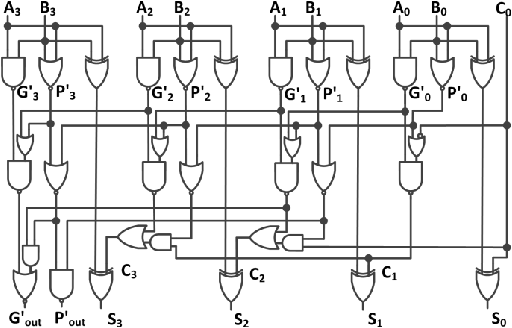
\includegraphics[scale=0.75]{figures/cla-4bit.png}
    \caption{Carry-LookAhead 4-Bit}
    \label{fig:cla-4bit}
\end{figure}

\section{Desenvolvimento}

\subsection{Propagation Generator}

O primeiro passo é projetar um módulo VHDL chamado "Propagation Generator" que determine se o carry será gerado ou propagado pelo somador de 4 bits "Carry-Lookahead". O módulo possui a seguinte interface:

\begin{lstlisting}
    ENTITY propagation_generator IS
    PORT (
        a, b : IN STD_LOGIC_VECTOR(3 DOWNTO 0);
        vec_p, vec_g : OUT STD_LOGIC_VECTOR(3 DOWNTO 0);
        p, g : OUT STD_LOGIC
    );
    END propagation_generator;
    
    ARCHITECTURE behavior OF propagation_generator IS
        SIGNAL p_vec, g_vec : STD_LOGIC_VECTOR(3 DOWNTO 0);
    BEGIN
        PROCESS (a, b)
        BEGIN
            p_vec <= a XOR b;
            g_vec <= a AND b;
        END PROCESS;
    
        vec_p <= p_vec;
        vec_g <= g_vec;
        p <= p_vec(3) AND p_vec(2) AND p_vec(1) AND p_vec(0);
        g <= g_vec(3) OR (g_vec(2) AND p_vec(3)) OR (p_vec(3) AND p_vec(2) AND g_vec(1)) OR (p_vec(3) AND p_vec(2) AND p_vec(1) AND g_vec(0));
    END behavior;
\end{lstlisting}

\subsection{LookAhead}

Com as informações sobre a propagação e a geração de carry do circuito, podemos calcular os carries de cada bit e realizar a soma em si. Criaremos o módulo VHDL "LookAhead4bit":

\begin{lstlisting}
    ENTITY LookAhead4Bit IS
    PORT(
        a, b, p, g : IN STD_LOGIC_VECTOR(3 DOWNTO 0);
        cin : IN STD_LOGIC;
        s : OUT STD_LOGIC_VECTOR(3 DOWNTO 0);
    );
    END LookAhead4Bit;
    
    ARCHITECTURE LookAhead4Bit OF LookAhead4Bit IS
    BEGIN
        s(0) <= p(0) XOR cin;
        s(1) <= p(1) XOR (g(0) OR (p(0) AND cin));
        s(2) <= p(2) XOR (g(1) OR (p(1) AND g(0)) OR (p(1) AND p(0) AND cin));
        s(3) <= p(3) XOR ((p(2) AND g(1)) OR (p(2) AND p(1) AND g(0)) OR (p(2) AND p(1) AND p(0) AND cin));
    END LookAhead4Bit;
\end{lstlisting}

\subsection{Carry Generator}

Para melhor modularização, criaremos o módulo VHDL "Carry Generator" responsável por calcular o "carry out" de dois somadores de 4 bits:

\begin{lstlisting}
    ENTITY carry_generator IS
    PORT (
        p1, g1, p2, g2, cin : IN STD_LOGIC;
        cout, c : OUT STD_LOGIC
    );
    END carry_generator;
    
    ARCHITECTURE behavior OF carry_generator IS
    
    BEGIN
        c <= g1 OR (p1 AND cin);
        cout <= g2 OR (p2 AND c) OR (p1 AND g2 AND cin);
    END behavior;
\end{lstlisting}

\subsection{4-Bit Carry-LookAhead}

Combinando os módulos anteriores, criaremos o somador de 4 bits "Carry-Lookahead". Para aumentar a capacidade do somador, basta conectar outros módulos de somadores de 4 bits, formando somadores de 8, 16 ou 32 bits.

\subsection{Output Size}

Agora, projetaremos o módulo "Output Size", que combinará todas as saídas de 4 bits em uma única saída de 32 bits, modularizando-a de acordo com o sinal de controle:

\begin{lstlisting}
    ENTITY output_size IS
    PORT (
        s0, s1, s2, s3, s4, s5, s6, s7 : IN STD_LOGIC_VECTOR(3 DOWNTO 0);
        sel : IN STD_LOGIC_VECTOR(1 DOWNTO 0);
        s : OUT STD_LOGIC_VECTOR(31 DOWNTO 0);
    );
    END output_size;
    
    ARCHITECTURE behavior OF output_size IS
        SIGNAL s_int : STD_LOGIC_VECTOR(31 DOWNTO 0);
    
    BEGIN
        s_int(3 DOWNTO 0) <= s0;
        s_int(7 DOWNTO 4) <= s1;
        s_int(11 DOWNTO 8) <= s2;
        s_int(15 DOWNTO 12) <= s3;
        s_int(19 DOWNTO 16) <= s4;
        s_int(23 DOWNTO 20) <= s5;
        s_int(27 DOWNTO 24) <= s6;
        s_int(31 DOWNTO 28) <= s7;
    
        PROCESS (sel)
        BEGIN
            CASE sel IS
                WHEN "00" =>
                    s(3 DOWNTO 0) <= s_int(3 DOWNTO 0);
                WHEN "01" =>
                    s(7 DOWNTO 0) <= s_int(7 DOWNTO 0);
                WHEN "10" =>
                    s(15 DOWNTO 0) <= s_int(15 DOWNTO 0);
                WHEN "11" =>
                    s <= s_int;
            END CASE;
        END PROCESS;
    END behavior;
\end{lstlisting}

\subsection{Signal Decoder}

Dado que a entrada também é de 32 bits, o módulo VHDL "Signal Decoder" é necessário para separar os sinais de cada grupo de 4 bits:

\begin{lstlisting}
    ENTITY signal_decoder IS
    PORT (
        a, b : IN STD_LOGIC_VECTOR(31 DOWNTO 0);
        a0, a1, a2, a3, a4, a5, a6, a7, b1, b2, b3, b4, b5, b6, b7 : OUT STD_LOGIC_VECTOR(3 DOWNTO 0);
    );
    END signal_decoder;
    
    ARCHITECTURE Behavioral OF signal_decoder IS
    
    BEGIN
        a0 <= a(3 DOWNTO 0);
        a1 <= a(7 DOWNTO 4);
        a2 <= a(11 DOWNTO 8);
        a3 <= a(15 DOWNTO 12);
        a4 <= a(19 DOWNTO 16);
        a5 <= a(23 DOWNTO 20);
        a6 <= a(27 DOWNTO 24);
        a7 <= a(31 DOWNTO 28);
    
        b1 <= b(3 DOWNTO 0);
        b2 <= b(7 DOWNTO 4);
        b3 <= b(11 DOWNTO 8);
        b4 <= b(15 DOWNTO 12);
        b5 <= b(19 DOWNTO 16);
        b6 <= b(23 DOWNTO 20);
        b7 <= b(27 DOWNTO 24);
    END Behavioral;
\end{lstlisting}

\subsection{Inverter}

Para realizar o complemento de 2, criaremos o módulo VHDL "Inverter", que, dependendo do sinal de controle, inverterá ou não os bits de um número:

\begin{lstlisting}
    ENTITY inverter IS
        PORT (
            a : IN STD_LOGIC_VECTOR(31 DOWNTO 0);
            sel : IN STD_LOGIC;
            s : OUT STD_LOGIC_VECTOR(31 DOWNTO 0);
        );
    END inverter;
    
    ARCHITECTURE behavior OF inverter IS
    BEGIN
        PROCESS (a, sel)
        BEGIN
            IF (sel = '1') THEN
                s <= NOT a;
            ELSE
                s <= a;
            END IF;
        END PROCESS;
    END behavior;
\end{lstlisting}

\section{Testes}

\begin{figure}[h]
    \centering
    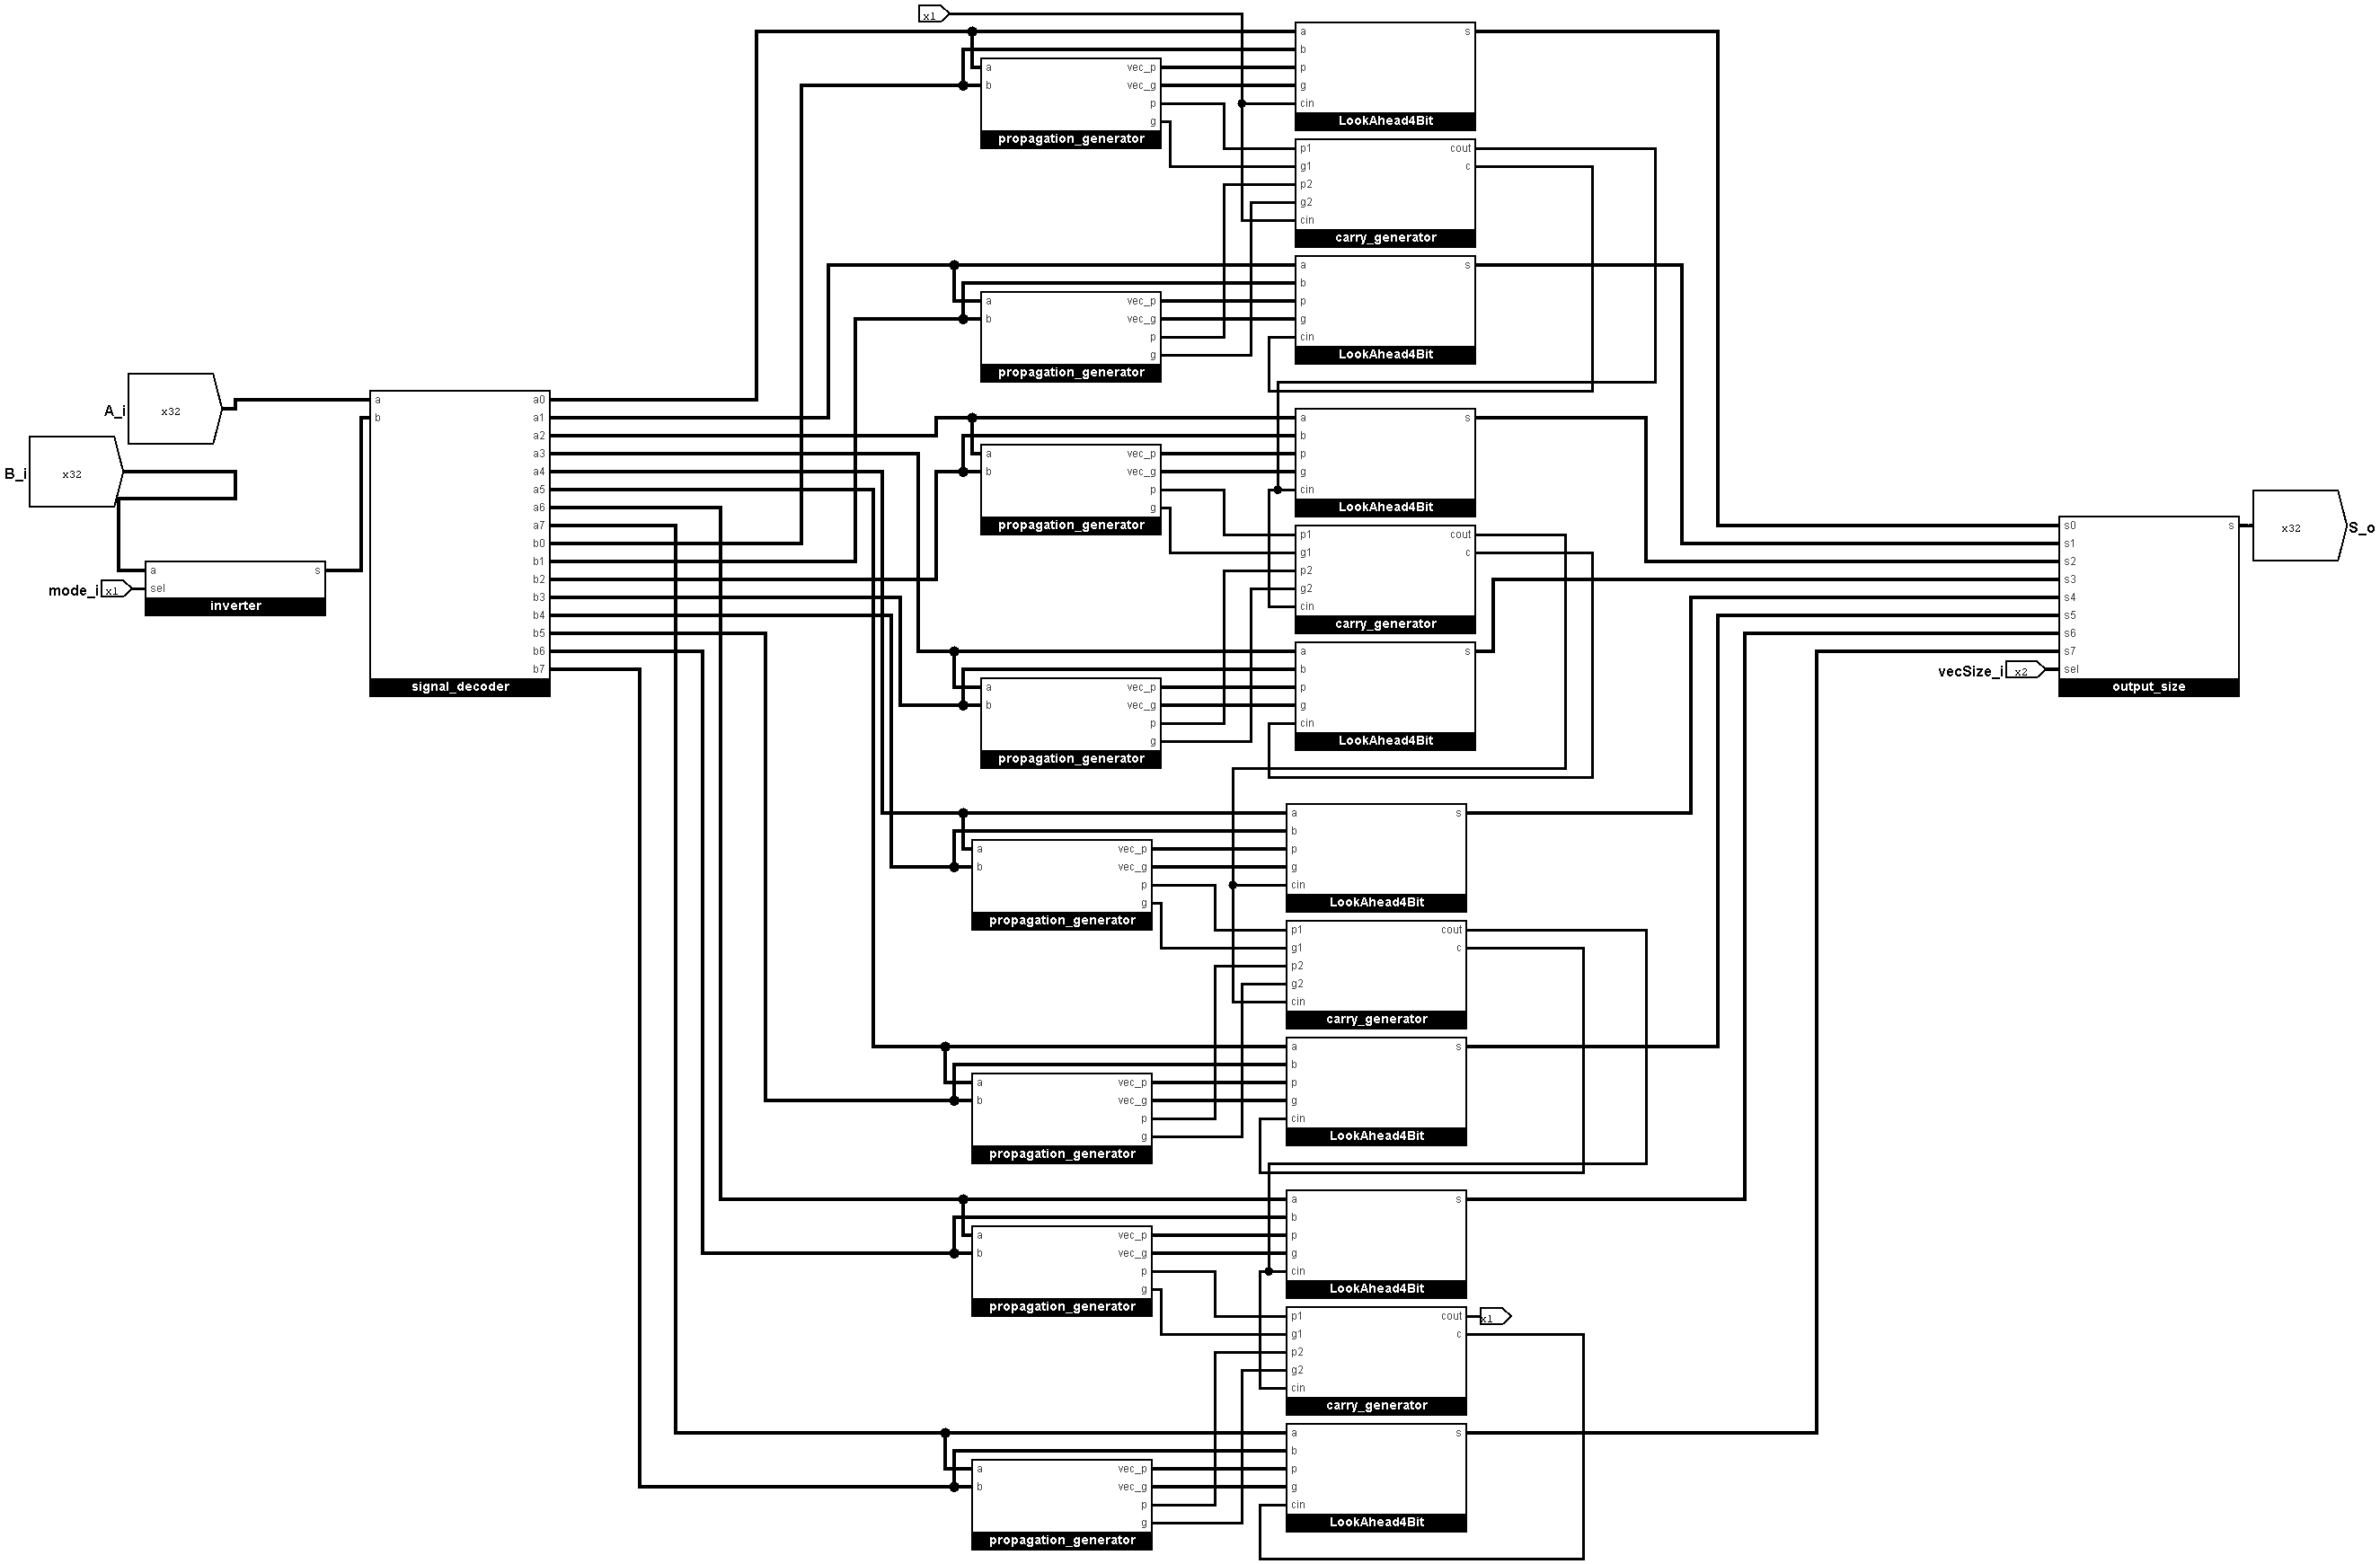
\includegraphics[scale=0.1875]{figures/32clas.png}
    \caption{32-Bit Carry-LookAhead Adder/Sub}
    \label{fig:32clas}
\end{figure}

Os testes serão realizados usando o testVector do LogiSim. O resultado será verificado para determinar se o circuito do somador de 32 bits funcionou corretamente.

\begin{table}
    \resizebox{\textwidth}{!}{%
    \begin{tabular}{|c|c|c|c|c|}
        \hline
        $A_i[32]$ & $B_i[32]$ & $mode_i[1]$ & $vecSize_i[2]$ & $S_o[32]$ \\
        \hline
        00000000000000000000000000000000 & 00000000000000000000000000000000 & 1 & 11 & 00000000000000000000000000000000 \\
        00000000000000000000000000000001 & 00000000000000000000000000000001 & 0 & 00 & 00000000000000000000000000000010 \\
        00000000000000000000000000000111 & 00000000000000000000000000000110 & 0 & 01 & 00000000000000000000000000000101 \\
        00000000000000000000000000011000 & 00000000000000000000000000001001 & 0 & 10 & 00000000000000000000000000000001 \\
        00000000000000000000000000111111 & 00000000000000000000000000101010 & 1 & 11 & 00000000000000000000000000010101 \\
        11111111111111111111111111110000 & 00000000000000000000000000001111 & 0 & 00 & 00000000000000000000000000000001 \\
        11111111111111111111111111111000 & 11111111111111111111111111110111 & 1 & 01 & 00000000000000000000000011111111 \\
        \hline
    \end{tabular}
    }
\end{table}

\section{Referências}

\begin{enumerate}
\item \textit{Computer Organization and Design RISC-V Edition: The Hardware Software Interface}, 2nd edition, by David A. Patterson and John L. Hennessy. Morgan Kaufmann, 2021.

\item \textit{Computer Organization and Architecture: Designing for Performance}, 11th edition, by William Stallings. Pearson, 2022.

\item \textit{Digital Design Using VHDL: A Systems Approach} by John F. Wakerly. Pearson, 2016.

\end{enumerate}

\end{document}